
%% Based on the style files for ACL-IJCNLP-2009, which were, in turn,
%% based on the style files for EACL-2009 and IJCNLP-2008...

%% Based on the style files for EACL 2006 by 
%%e.agirre@ehu.es or Sergi.Balari@uab.es
%% and that of ACL 08 by Joakim Nivre and Noah Smith

\documentclass[11pt,letterpaper]{article}
\usepackage{naaclhlt2013}
\usepackage{times}
\usepackage{url}
\usepackage{latexsym}
\usepackage[english]{babel}
%\setlength\titlebox{6.5cm}    % You can expand the title box if you
% really have to
\usepackage{graphicx}
\usepackage{placeins}

\title{WSD2: Parameter optimisation for Memory-based Cross-Lingual Word-Sense Disambiguation}

\author{Maarten van Gompel and Antal van den Bosch \\
  Centre for Language Studies, Radboud University Nijmegen \\
  {\tt proycon@anaproy.nl}, {\tt a.vandenbosch@let.ru.nl}}

%\date{}

\begin{document}
\maketitle
\begin{abstract}
We present our system WSD2 which participated in the Cross-Lingual Word-Sense Disambiguation task for SemEval 2013 \cite{TASKPAPER}. The system closely resembles our winning system for the same task in SemEval 2010. It is based on $k$-nearest neighbour classifiers which map words with local and global context features onto their translation, i.e. their cross-lingual sense. The system participated in the task for all five languages and obtained winning scores for four of them when asked to predict the best translation(s). We tested various configurations of our system, focusing on various levels of hyperparameter optimisation and feature selection. Our final results indicate that hyperparameter optimization did not lead to the most optimal results, indicating overfitting by our optimisation method in this aspect. Feature selection does have a modest positive impact.
\end{abstract}


\section{Introduction}

WSD2 is a rewrite and extension of our previous system \cite{WSD1} that participated in the Cross-Lingual Word Sense Disambiguation task in SemEval 2010 \cite{WSD}. In WSD2 we introduce and test a new level of hyperparameter optimisation. Unlike the previous occasion, we participate in all five target languages (Dutch, Spanish, Italian, French, and German). The task presents twenty polysemous nouns with fifty instances each to be mapped onto normalized (lemmatized) translations in all languages. The task is described in detail by \newcite{TASKPAPER}.

Trial data is provided and has been used to optimise system parameters. Due to the unsupervised nature of the task, no training data is provided. However, given that the gold standard of the task is based exclusively on the Europarl parallel corpus \cite{Europarl}, we select that same corpus to minimise our chances of delivering translations that the human annotators preparing the test data could have never picked.
   
The system may output several senses per instance, rather than producing just one sense prediction. These are evaluated in two different ways. The scoring type ``\textbf{best}'' expects that the system outputs the sense it considers the most likely, or a number of senses in the order of its confidence in these senses being correct. Multiple guesses are penalised, however. In contrast, the scoring type ``\textbf{out of five}'' expects five guesses, in which each answer carries the same weight. These metrics are more extensively described in \newcite{CLLS} and \newcite{TASKPAPER}. 

\section{System Description}

The WSD2 system, like its predecessor, distributes the task over word experts. Each word expert is a $k$-nearest neighbour classifier specialising in the disambiguation of a single of the twenty provided nouns. This is implemented using the Tilburg Memory Based Learner (TiMBL) \cite{TIMBL}. The classifiers are trained as follows: First the parallel corpus which acts as training data is tokenised using Ucto \cite{UCTO}, for all five language pairs. Then, a word-alignment between sentence pairs in the Europarl training data is established, for which we use GIZA++ \cite{GIZA}. We use the intersection of both translation directions, as we know the sense repository from which the human annotators preparing the task's test data can select their translations is created in the same fashion. 

Whilst the word alignment is computed on the actual word forms, we also need lemmas for both the source language (English) as well as for all of the five target languages. The English nouns in the test data can be either singular or plural, and both forms may occur in the input. Second, the target translations all have to be mapped to their lemma forms. Moreover, to be certain we are dealing with nouns in the source language, a Part-of-Speech tagger is also required. PoS tagging and lemmatisation is conducted using Freeling \cite{FREELING} for English, Spanish and Italian; Frog \cite{TADPOLE} for Dutch, and TreeTagger \cite{TREETAGGER} for German and French. 

With all of this data generated, we then iterate over all sentences in the parallel corpus and extract occurrences of any of the twenty nouns, along with the translation they are aligned to according to the word alignment. We extract the words themselves and compute the lemma and the part-of-speech tag, and do the same for a specified number of words to the left and to the right of the found occurrence. These constitute the {\em local context}\/ features. 

In addition to this, {\em global context}\/ features are extracted; these are a set of keywords per lemma and per translation which are found occurring above certain occurrence thresholds at arbitrary positions in the same sentence, as this is the widest context supplied in the task data. The global context features are represented as a binary bag-of-words model in which the presence of each of the keywords that may be indicative for a given mapping of the focus word to a sense is represented by a boolean value. Such a set of keywords is constructed for each of the twenty nouns, per language.

%<very close paraphrase from earlier paper>
The method used to extract these keywords ($k$) is proposed by \newcite{NgL96} and used also by \newcite{Hoste+02}. Assume we have a focus word $f$, more precisely, a lemma of one of the target nouns. We also have one of its aligned translations/senses $s$, also a lemma. We can now estimate $P(s|k)$, the probability of sense $s$, given a keyword $k$, by dividing $N_{s,k_{local}.}$ (the number of occurrences of a possible local context word $k$ with particular focus word lemma-PoS combination and with a particular sense $s$) by $N_{k_{local}}$ (the number of occurrences of a possible local context keyword $k_{loc}$ with a particular focus word-PoS combination regardless of its sense). If we also take into account the frequency of a possible keyword $k$ in the complete training corpus ($N_{k_{corpus}}$), we get:

\begin{equation}
P(s|k) = \frac{N_{s,k_{local}}}{N_{k_{local}}}(\frac{1}{N_{k_{corpus}}})
\end{equation}

\newcite{Hoste+02} select a keyword $k$ for inclusion in the bag-of-words representation if that keyword occurs more than $T_1$ times in that sense $s$, and if $P(s|k) \ge T_2$. Both $T_1$ and $T_2$ are predefined thresholds, which by default were set to $3$ and $0.001$ respectively. In addition, WSD2 and its predecessor WSD1 contain an extra parameter which can be enabled to automatically adjust the $T_1$ threshold when it yields too many or too few keywords. The selection of bag-of-word features is computed prior to the extraction of the training instances, as this information is a prerequisite for the successful generation of both training and test instances. 
%</very close paraphrase from earlier paper> 

\section{Feature and Hyperparameter Optimisation}

The size of the local context, the inclusion of global context features, and the inclusion of syntactic features are all feature selection choices to the system, allowing for a variety of combinations to be tested. In addition, each word expert is a $k$-nearest neighbour classifier that can take on many hyperparameters beyond $k$. In the present study we performed both optimisations for all word experts, but the optimisations were performed independently to reduce complexity: we optimised classifier hyperparameters on the basis of the training examples extracted from our parallel corpus, producing optimal accuracy on each word-expert. We optimised feature selection on the basis of the trial data provided for the task. As has been argued before \cite{Hoste+02}, the joint search space of feature selection and hyperparameters is prohibitively large. Our current setup runs the risk of finding hyperparameters that are not optimal for the feature selection selected in the second optimisation step. Our final results indeed show that only feature selection produced improved results. We choose the feature selection with the highest score on the trial set, for each of the nouns and separately for both evaluation metrics in the task.

To optimise the choice of hyperparameters per word expert, a heuristic parameter search algorithm \cite{PARAMSEARCH} was used that implements wrapped progressive sampling using cross-validation: it performs a large number of experiments with many hyperparameter setting combinations on small samples of training data, and then progressively zooms in on combinations estimated to perform well with larger samples of the training data. As a control run we also trained word experts with default hyperparameters\footnote{i.e. with $k=1$ and with all other hyperparameters at their default values as specified in the TiMBL implementation}.


\section{Experiments \& Results}

To assess the accuracy of a certain configuration of our system as a whole, we take the average over all word experts. An initial experiment on the trial data explores the impact of different context sizes, with hyperparameter optimisation on the classifiers. The results, shown in Figure~\ref{figcontext}, clearly indicate that on average the classifiers perform best with a local context of just one word to the left and one to the right of the word to be disambiguated. Larger context sizes have a negative impact on average accuracy. These tests include hyperparameter optimisation, but the same result holds without.

\begin{figure}[t]
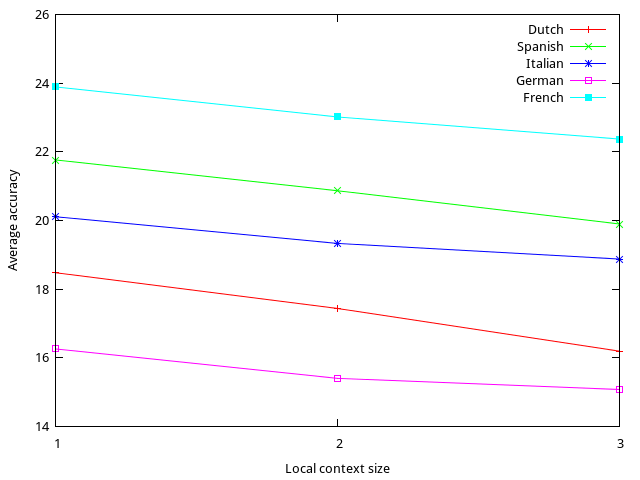
\includegraphics[width=8cm]{context.png}
\caption{Average accuracy for different local context sizes}
\label{figcontext}
\end{figure}

We submitted three configurations of our system to the shared task, the maximum number of runs. Adding lemma features to the local context window of three words proves beneficial in general, as shown in Table~\ref{tabtrialresults}. This is therefore the first configuration we submitted (\texttt{c1l}). As second configuration (\texttt{c1lN}) we submitted the same configuration without parameter optimisation on the classifiers.

\begin{table}[t]
\footnotesize
\begin{tabular}{|l|r|r|r|r|r|}
\hline
\textbf{BEST} & \textbf{ES} & \textbf{FR} & \textbf{IT} & \textbf{NL} & \textbf{DE} \\
\hline
baseline &  19.65 & 21.23 & 15.17 & 15.75 & 13.16 \\
\hline
plain & 21.76 & 23.89 & 20.10 & 18.47 & 16.25 \\
$+$lem (\texttt{c1l}) & 21.88 & \textbf{23.93} & \textbf{19.90} & \textbf{18.61} & \textbf{16.43} \\
$+$pos & 22.09 & 23.91 & 19.95 & 18.02 & 15.37 \\
lem$+$pos & \textbf{22.12} & 23.61 & 19.82 & 18.18 & 15.48 \\
\hline
glob.context & 20.57 & 23.34 & 17.76 & 17.06 & 16.05 \\
\hline
\textbf{OUT-OF-5} & \textbf{ES} & \textbf{FR} & \textbf{IT} & \textbf{NL} & \textbf{DE} \\
\hline
baseline & 48.34 & 45.99 & 34.51 & 38.59 & 32.90 \\
\hline
plain & 49.81 & \textbf{50.91} & 42.30 & 41.74 & \textbf{36.86} \\
$+$lem (\texttt{c1l}) & \textbf{49.91} & 50.65 & \textbf{42.41} & \textbf{41.83} & 36.45 \\
$+$pos & 47.86 & 49.72 & 41.91 & 41.31 & 35.93 \\
lem$+$pos & 47.90 & 49.75 & 41.49 & 41.31 & 35.80 \\
\hline
glob.ccontext & 48.09 & 49.68 & 40.87 & 37.70 & 34.47 \\
\hline
\end{tabular}
\caption{Feature exploration on the trial data}
\label{tabtrialresults}
\end{table}

The third configuration (\texttt{var}) we submitted includes feature selection, and selects per word expert the configuration that has the highest score on the trial data, and thus tests all kinds of configurations. Note that hyperparameter optimisation is also enabled for this configuration. Due to the feature selection on the trial data, we by definition obtain the highest scores on this trial data, but this carries the risk of overfitting. Results on the trial data are shown in Table~\ref{tabpar}.

\begin{table}
\footnotesize
\begin{tabular}{|l|r|r|r|r|r|}
\hline
\textbf{BEST} & \textbf{ES} & \textbf{FR} & \textbf{IT} & \textbf{NL} & \textbf{DE} \\
\hline
c1lN & 22.60  & 24.09 & 19.87 & 18.70 & 16.43 \\ 
c1l & 21.88 & 23.93 & 19.90 & 18.61 & 16.43 \\ 
var & 23.79 & \textbf{25.66} & \textbf{21.65} & \textbf{20.19} & \textbf{19.06} \\
varN & \textbf{23.90} &  25.65 & 21.52 & 19.92 & 18.96 \\ 
\hline
\textbf{OUT-OF-5} &  \textbf{ES} & \textbf{FR} & \textbf{IT} & \textbf{NL} & \textbf{DE} \\
\hline
c1lN & 50.14 & 50.98 & 42.92 & 42.08 &  36.45 \\
c1l & 49.91 & 50.65 & 42.41 & 41.83 & 36.45 \\ 
var & 51.95 & \textbf{53.66} & 45.59 & \textbf{44.66} & \textbf{39.81} \\
varN & \textbf{52.91} & 53.61 & \textbf{45.92} & 44.32 & 39.40 \\
\hline
\end{tabular}
\caption{Results on the trial data}
\label{tabpar}
\end{table}
 
The hyperparameter optimisation, optimised on classifier accuracy, has a slightly negative impact, suggesting overfitting on the training data. Therefore a fourth configuration (\texttt{varN}) was tried later to independently assess the idea of feature selection, without hyperparameter optimisation on the classifiers. This proves to be a good idea. However, the fourth configuration was not yet available for the actual competition. This incidentally would have had no impact on the final ranking between competitors. When we run these systems on the actual test data of the shared task, we obtain the results in Table~\ref{tabfinal}. The best score amongst the other competitors is mentioned in the last row for reference, this is participant Alex Rudnick for all but Best-Spanish.

\begin{table}[tbh]
\footnotesize
\begin{center}
\begin{tabular}{|l|r|r|r|r|r|}
\hline
\textbf{BEST} & \textbf{ES} & \textbf{FR} & \textbf{IT} & \textbf{NL} & \textbf{DE} \\
\hline
baseline & 23.23 & 25.74 & 20.21 & 20.66 & 17.42 \\ 
\hline
c1l &  28.40 & 29.88 & 25.43 & 23.14 & 20.70 \\
c1lN &  28.65 & 30.11 & \textbf{25.66} & \textbf{23.61} & 20.82 \\
var & 23.3 & 25.89 & 20.38 & 17.17 & 16.2 \\
varN & 29.05 & \textbf{30.15} & 24.90 & 23.57 & \textbf{21.98} \\
best.comp & \textbf{32.16} & 28.23 & 24.62 & 22.36 & 19.92 \\ 
\hline
\textbf{OUT-OF-5} & \textbf{ES} & \textbf{FR} & \textbf{IT} & \textbf{NL} & \textbf{DE} \\
\hline
baseline & 53.07 & 51.36 & 42.63 & 43.59 & 38.86 \\
\hline
c1l &  58.23 & 59.07 & 52.22 & \textbf{47.83} & 43.17 \\
c1lN & 57.62 & \textbf{59.80} & 52.73 & 47.62 & 43.24 \\
var & 55.70 & 59.19 & 51.18 & 46.85 & 41.46 \\
varN & 58.61 & 59.26 & 50.89 & 50.42 & 43.34 \\
best.comp & \textbf{61.69} & 58.20 & \textbf{53.57}  & 46.55 & \textbf{43.66} \\ 
\hline
\end{tabular}
\end{center}
\caption{Results on the test set}
\label{tabfinal}
\end{table}

A major factor in this task is the accuracy of lemmatisation, and to lesser extent of part-of-speech tagging. We conducted additional experiments on German and French without lemmatisation, tested on on the trial data. Results immediately fell below baseline. 

Another main factor is the quality of the word alignments, and the degree to which the found word alignments correspond with the translations the human annotators could choose from in preparing the gold standard. An idea we tested is, instead of relying on the mere intersection of word alignments, to use a phrase-translation table generated by and for the Statistical Machine Translation system Moses \cite{Koehn+07}, which uses the grow-diag-final heuristic to extract phrase pairs. This results in more phrases, and whilst this is a good idea for MT, in the current task it has a detrimental effect, as it creates too many translation options and we do not have an MT decoder to discard ineffective options in this task. The grow-diag-final heuristic tends to incorporate unaligned words to the end of a translation in the translation option, which for our purposes is a bad idea. % voeg een referentie naar Koehn toe

\section{Conclusion}

In this study we have taken parameter optimisation one step further compared to our previous research \cite{WSD1}, namely by selecting system parameters per word expert from the best configurations on the trial data. Optimising the hyperparameter of the classifiers on the training data proves to have a slightly negative effect, especially when combined with the selection of features. This is likely due to the fact that feature selection was performed after hyperparameter optimisation, causing certain optimisations to be rendered ineffective.

We can furthermore uphold the conclusion from previous research that including lemma features is generally a good idea. As to the number of local context features, we observed that a context size of one feature to the left, and one to the right, has the best overall average accuracy. Eventually, due to our feature selection without hyperparameter optimisation on the classifier not being available yet at the time of submission, our simplest system \texttt{c1lN} emerged as best in the contest.

When asked to predict the best translation(s), our system comes out on top for four out of five languages; only for Spanish we are surpassed by two competitors. Our out-of-five predictions win for two out of five languages, and are fairly close the the best competitor for the others, except again for Spanish.   

We assumed independence between hyperparameter optimisation and feature selection, where the former was conducted using cross-validation on the training data rather than on the development set. As this independence assumption is a mere simplification to reduce algorithmic complexity, future research could focus on a more integrated approach and test hyperparameter optimisation of the classifiers on the trial set. It is conceivable that hyperparameter optimisation of the classifiers could prove beneficial then. 

The WSD2 system is available as open-source under the GNU Public License v3. It is implemented in Python \cite{PYTHON} and can be obtained from http://github.com/proycon/wsd2\footnote{git commit f10e796141003d8a2fbaf8c463588a6d7380c05e represents a fair state of the system at the time of submission}. The experimental data and results are included in the git repository as well.  

\bibliographystyle{naaclhlt2013}
\bibliography{semeval2013_wsd2}

\end{document}
